\documentclass{article}
\usepackage{amsmath, amsthm, amssymb}
\usepackage{graphicx}
\usepackage{hyperref}      % Para hipervínculos
\usepackage{geometry}
\usepackage{multicol}
\usepackage{array}
\usepackage{listings}
\usepackage{comment}
\usepackage{xcolor}
\usepackage{verse}
\geometry{a4paper, left=20mm, right=20mm, top=20mm, bottom=20mm}


% Definir márgenes de la página para evitar desbordamientos
\geometry{a4paper, margin=1in}

% Definir el estilo de los códigos en C++
\lstdefinestyle{cpp}{
    language=C++, 
    backgroundcolor=\color{white}, 
    basicstyle=\ttfamily\footnotesize, 
    breaklines=true,               % Hacer que el código se divida automáticamente
    breakatwhitespace=true,        % Romper las líneas solo en espacios
    keywordstyle=\color{blue},
    commentstyle=\color{lightgray},
    stringstyle=\color{red},
    showstringspaces=false,
    xleftmargin=10pt,              % Margen izquierdo
    xrightmargin=10pt,             % Margen derecho
    frame=single                   % Agregar borde al código
}

\title{Apuntes Algoco}
\author{Marco Repetto y Oscar Ruiz}
\date{}

\begin{document}
\maketitle


% Centrar el contenido en la página
\vspace*{\fill} % Espacio flexible desde arriba
\begin{center}
{\Large % Texto del poema en tamaño grande
Dios te salve, María, \\
llena eres de gracia; \\
el Señor es contigo. \\
Bendita Tú eres \\
entre todas las mujeres, \\
y bendito es el fruto de tu vientre, Jesús. \\
Santa María, Madre de Dios, \\
ruega por nosotros, pecadores, \\
ahora y en la hora de nuestra muerte. Amén.
}
\end{center}
\vspace*{\fill} % Espacio flexible hacia abajo
\newpage
\tableofcontents







\newpage

% Incluye cada sección en el documento principal
\section{Plantillas}
\subsection{Estructura Base para Problemas de Algoritmos}

\begin{lstlisting}[style=cpp]
#include <algorithm>
#include <bits/stdc++.h>
using namespace std;

#define INF numeric_limits<int>::max()
#define MINF numeric_limits<int>::min()
#define pb push_back
#define pp pop_back
#define all(v) (v).begin(), (v).end()
#define fast_io ios::sync_with_stdio(false); cin.tie(nullptr);

typedef long long ll;
typedef pair<int, int> pii;

\end{lstlisting}


\subsection{Plantilla para Fuerza Bruta}

\begin{lstlisting}[style=cpp]
// Fuerza Bruta: Generar todas las combinaciones posibles
void fuerzaBruta(const vector<int>& nums) {
    int n = nums.size();
    for (int mask = 0; mask < (1 << n); ++mask) {
        vector<int> subset;
        for (int i = 0; i < n; ++i) {
            if (mask & (1 << i)) subset.pb(nums[i]);
        }
        // Procesar el subset generado
        for (int x : subset) cout << x << " ";
        cout << endl;
    }
}


\end{lstlisting}

\subsection{Plantilla para Programacion Dinamica}

\begin{lstlisting}[style=cpp]
// Memoizacion (Top-Down)
map<pair<int, int>, int> memo;

int DP(int i, int j) {
    if (i == 0 || j == 0) return 0; // Caso base
    if (memo.find({i, j}) != memo.end()) return memo[{i, j}];
    
    // Supongamos que el problema requiere comparar dos indices
    int result = max(DP(i - 1, j), DP(i, j - 1));
    memo[{i, j}] = result;
    return result;
}

// Tabla Iterativa (Bottom-Up)
int DP_iterative(const vector<int>& nums) {
    int n = nums.size();
    vector<vector<int>> dp(n + 1, vector<int>(n + 1, 0));
    for (int i = 1; i <= n; ++i) {
        for (int j = 1; j <= n; ++j) {
            dp[i][j] = max(dp[i - 1][j], dp[i][j - 1]);
        }
    }
    return dp[n][n];
}


\end{lstlisting}

\subsection{Plantilla para Algoritmos Greedy}

\begin{lstlisting}[style=cpp]
int greedy(vector<int>& nums) {
    sort(all(nums)); // Ordenar para facilitar decisiones
    int result = 0;
    for (int i = 0; i < nums.size(); ++i) {
        result += nums[i]; // O cualquier logica greedy
    }
    return result;
}
\end{lstlisting}

\subsection{Plantilla para Backtracking}

\begin{lstlisting}[style=cpp]
void backtracking(vector<int>& nums, vector<int>& solution, vector<bool>& used) {
    if (solution.size() == nums.size()) {
        // Procesar solucion valida
        for (int x : solution) cout << x << " ";
        cout << endl;
        return;
    }
    for (int i = 0; i < nums.size(); ++i) {
        if (!used[i]) {
            used[i] = true;
            solution.pb(nums[i]);
            backtracking(nums, solution, used);
            solution.pop_back();
            used[i] = false;
        }
    }
}



\end{lstlisting}

\subsection{Plantilla para Dividir y Conquistar}

\begin{lstlisting}[style=cpp]
int divideYConquista(const vector<int>& nums, int l, int r) {
    if (l == r) return nums[l]; // Caso base
    int mid = l + (r - l) / 2;
    int left = divideYConquista(nums, l, mid);
    int right = divideYConquista(nums, mid + 1, r);
    return max(left, right); // Combinar resultados
}
\end{lstlisting}

\section{Estructuras de datos}
\label{sec:estructuras_de_datos}

\subsection{std::array}
\label{subsec:std_array}
Contenedor de tamaño fijo. 

\subsubsection{Formas de definirlo:}
\begin{itemize}
  \item Syntaxis genérica: \texttt{type name [size];}
  \item Inicializar con ceros: \texttt{int baz [5] = \{ \};}
  \item Inicializar con valores: \texttt{int foo [5] = \{ 16, 2, 77, 40, 12071 \};}
\end{itemize}

\subsection{std::vector}
\label{subsec:std_vector}
Contenedor dinámico de tamaño variable.

\subsubsection{Formas de definirlo:}
\begin{itemize}
  \item Syntaxis genérica: \texttt{std::vector<type> name;}
  \item Inicializar con ceros: \texttt{std::vector<int> baz (5);}
  \item Inicializar con valores: \texttt{std::vector<int> foo \{ 16, 2, 77, 40, 12071 \};}
\end{itemize}

\subsubsection{Funciones miembro:}
\begin{itemize}
  \item \texttt{push\_back(value)}: Agrega un elemento al final [O(1)].
  \item \texttt{pop\_back()}: Elimina el último elemento [O(1)].
  \item \texttt{size()}: Retorna la cantidad de elementos [O(1)].
  \item \texttt{empty()}: Retorna \texttt{true} si está vacío [O(1)].
  \item \texttt{clear()}: Elimina todos los elementos [O(n)].
  \item \texttt{front()}: Retorna el primer elemento [O(1)].
  \item \texttt{back()}: Retorna el último elemento [O(1)].
  \item \texttt{insert(iterator, value)}: Inserta un elemento en la posición indicada [O(n)].
\end{itemize}

\subsection{std::list}
\label{subsec:std_list}
Contenedor de secuencia que permite inserciones y eliminaciones en cualquier posición en tiempo constante. 

\subsubsection{Formas de definirlo:}
\begin{itemize}
  \item Syntaxis genérica: \texttt{std::list<type> name;}
\end{itemize}

\subsubsection{Funciones miembro:}
\begin{itemize}
  \item \texttt{push\_back(value)}: Agrega un elemento al final [O(1)].
  \item \texttt{push\_front(value)}: Agrega un elemento al principio [O(1)].
  \item \texttt{pop\_back()}: Elimina el último elemento [O(1)].
  \item \texttt{pop\_front()}: Elimina el primer elemento [O(1)].
  \item \texttt{size()}: Retorna la cantidad de elementos [O(n)].
  \item \texttt{empty()}: Retorna \texttt{true} si está vacío [O(1)].
  \item \texttt{clear()}: Elimina todos los elementos [O(n)].
  \item \texttt{front()}: Retorna el primer elemento [O(1)].
  \item \texttt{back()}: Retorna el último elemento [O(1)].
  \item \texttt{insert(iterator, value, r)}: Inserta un elemento en la posición indicada [O(r)].
  \item \texttt{erase(iterator)}: Elimina el elemento en la posición indicada [O(1)]. 
\end{itemize}

\subsection{std::stack}
\label{subsec:std_stack}
Contenedor de tipo LIFO (Last In, First Out). 

\subsubsection{Formas de definirlo:}
\begin{itemize}
  \item Syntaxis genérica: \texttt{std::stack<type> name;}
\end{itemize}

\subsubsection{Funciones miembro:}
\begin{itemize}
  \item \texttt{push(value)}: Agrega un elemento al tope [O(1)].
  \item \texttt{pop()}: Elimina el elemento del tope [O(1)].
  \item \texttt{top()}: Retorna el elemento del tope [O(1)].
  \item \texttt{size()}: Retorna la cantidad de elementos [O(1)].
  \item \texttt{empty()}: Retorna \texttt{true} si está vacío [O(1)]. 
\end{itemize}

\subsection{std::queue}
\label{subsec:std_queue}
Contenedor de tipo FIFO (First In, First Out). 

\subsubsection{Formas de definirlo:}
\begin{itemize}
  \item Syntaxis genérica: \texttt{std::queue<type> name;}
\end{itemize}

\subsubsection{Funciones miembro:}
\begin{itemize}
  \item \texttt{push(value)}: Agrega un elemento al final [O(1)].
  \item \texttt{pop()}: Elimina el primer elemento [O(1)].
  \item \texttt{front()}: Retorna el primer elemento [O(1)].
  \item \texttt{back()}: Retorna el último elemento [O(1)].
  \item \texttt{size()}: Retorna la cantidad de elementos [O(1)].
  \item \texttt{empty()}: Retorna \texttt{true} si está vacío [O(1)]. 
\end{itemize}

\subsection{std::priority\_queue}
\label{subsec:std_priority_queue}
Cola de prioridad. Su funcionamiento es similar a una cola, pero los elementos son extraídos en orden de prioridad. Para definirla hay que especificar el tipo de dato y el contenedor que se usará internamente y el comparador (\ref{subsec:comparador}).

\subsubsection{Formas de definirlo:}
\begin{itemize}
  \item Syntaxis genérica: \texttt{std::priority\_queue<type> name;}
  \item Syntaxis con comparador: \texttt{std::priority\_queue<type, std::vector<type>, std::greater<type>> name;}
\end{itemize}

\subsection{std::set}
\label{subsec:std_set}
% Explicacion
Contenedor que almacena elementos únicos ordenados. 

\subsubsection{Formas de definirlo:}
\begin{itemize}
  \item Syntaxis genérica: \texttt{std::set<type> name;}
  \item Con comparador: \texttt{std::set<type, comp> name;}
\end{itemize}

\subsubsection{Funciones miembro:}
\begin{itemize}
  \item \texttt{insert(value)}: Inserta un elemento [O(log n)]. 
  \item \texttt{erase(value)}: Elimina el elemento con valor 'value' [O(log n)].
  \item \texttt{erase(iterator)}: Elimina el elemento en la posición indicada [O(1)].
  \item \texttt{erase(first, last)}: Elimina los elementos en el rango [O(n)].
  \item \texttt{find(value)}: Retorna un iterador al elemento con valor 'value' [O(log n)]. 
  \item \texttt{count(value)}: Retorna la cantidad de elementos con valor 'value' [O(log n)]. 
  \item \texttt{size()}: Retorna la cantidad de elementos [O(1)]. 
  \item \texttt{empty()}: Retorna \texttt{true} si está vacío [O(1)]. 
  \item \texttt{clear()}: Elimina todos los elementos [O(n)]. 
\end{itemize}

\subsection{std::unordered\_set}
\label{subsec:std_unordered_set}
% Explicacion
Contenedor que almacena elementos únicos sin ordenar. 

\subsubsection{Formas de definirlo:}
\begin{itemize}
  \item Syntaxis genérica: \texttt{std::unordered\_set<type> name;}
  \item Con comparador: \texttt{std::unordered\_set<type, comp> name;}
\end{itemize}

\subsubsection{Funciones miembro:}
\begin{itemize}
  \item \texttt{insert(value)}: Inserta un elemento [O(log n)]. 
  \item \texttt{erase(value)}: Elimina el elemento con valor 'value' [O(log n)].
  \item \texttt{erase(iterator)}: Elimina el elemento en la posición indicada [O(1)].
  \item \texttt{erase(first, last)}: Elimina los elementos en el rango [O(n)].
  \item \texttt{find(value)}: Retorna un iterador al elemento con valor 'value' [O(log n)]. 
  \item \texttt{count(value)}: Retorna la cantidad de elementos con valor 'value' [O(log n)]. 
  \item \texttt{size()}: Retorna la cantidad de elementos [O(1)]. 
  \item \texttt{empty()}: Retorna \texttt{true} si está vacío [O(1)]. 
  \item \texttt{clear()}: Elimina todos los elementos [O(n)]. 
\end{itemize}

\subsection{std::map}
\label{subsec:std_map}
% Explicacion
Contenedor que almacena pares clave-valor ordenados por la clave. La función del comparador es comparar las claves de los elementos, esto sirve para mantener el orden de los elementos.

\subsubsection{Formas de definirlo:}
\begin{itemize}
  \item Syntaxis genérica: \texttt{std::map<key, value> name;}
  \item Con comparador: \texttt{std::map<key, value, comp> name;}
\end{itemize}

\subsubsection{Funciones miembro:}
\begin{itemize}
  \item \texttt{operator[key]}: Retorna el valor asociado a la clave 'key' [O(log n)].
  \item \texttt{insert(pair)}: Inserta un par clave-valor [O(log n)]. 
  \item \texttt{erase(key)}: Elimina el elemento con clave 'key' [O(log n)].
  \item \texttt{erase(iterator)}: Elimina el elemento en la posición indicada [O(1)].
  \item \texttt{erase(first, last)}: Elimina los elementos en el rango [O(n)].
  \item \texttt{find(key)}: Retorna un iterador al elemento con clave 'key' [O(log n)]. 
  \item \texttt{count(key)}: Retorna la cantidad de elementos con clave 'key' [O(log n)]. 
  \item \texttt{size()}: Retorna la cantidad de elementos [O(1)]. 
  \item \texttt{empty()}: Retorna \texttt{true} si está vacío [O(1)]. 
  \item \texttt{clear()}: Elimina todos los elementos [O(n)]. 
\end{itemize}

\subsection{std::unordered\_map}
\label{subsec:std_unordered_map}
% Explicacion
Contenedor que almacena pares clave-valor sin ordenar. 

\subsubsection{Formas de definirlo:}
\begin{itemize}
  \item Syntaxis genérica: \texttt{std::unordered\_map<key, value> name;}
  \item Con comparador: \texttt{std::unordered\_map<key, value, comp> name;}
\end{itemize}

\subsubsection{Funciones miembro:}
\begin{itemize}
  \item \texttt{operator[key]}: Retorna el valor asociado a la clave 'key' [O(log n)].
  \item \texttt{insert(pair)}: Inserta un par clave-valor [O(log n)]. 
  \item \texttt{erase(key)}: Elimina el elemento con clave 'key' [O(log n)].
  \item \texttt{erase(iterator)}: Elimina el elemento en la posición indicada [O(1)].
  \item \texttt{erase(first, last)}: Elimina los elementos en el rango [O(n)].
  \item \texttt{find(key)}: Retorna un iterador al elemento con clave 'key' [O(log n)]. 
  \item \texttt{count(key)}: Retorna la cantidad de elementos con clave 'key' [O(log n)]. 
  \item \texttt{size()}: Retorna la cantidad de elementos [O(1)]. 
  \item \texttt{empty()}: Retorna \texttt{true} si está vacío [O(1)]. 
  \item \texttt{clear()}: Elimina todos los elementos [O(n)]. 
\end{itemize}

\subsection{std::deque}
\label{subsec:std_deque}
% Explicacion
Contenedor de secuencia que permite inserciones y eliminaciones en cualquier posición en tiempo constante.

\subsubsection{Formas de definirlo:}
\begin{itemize}
  \item Syntaxis genérica: \texttt{std::deque<type> name;}
\end{itemize}

\subsubsection{Funciones miembro:}
\begin{itemize}
  \item \texttt{push\_back(value)}: Agrega un elemento al final [O(1)].
  \item \texttt{push\_front(value)}: Agrega un elemento al principio [O(1)].
  \item \texttt{pop\_back()}: Elimina el último elemento [O(1)].
  \item \texttt{pop\_front()}: Elimina el primer elemento [O(1)].
  \item \texttt{size()}: Retorna la cantidad de elementos [O(1)].
  \item \texttt{empty()}: Retorna \texttt{true} si está vacío [O(1)].
  \item \texttt{clear()}: Elimina todos los elementos [O(n)].
  \item \texttt{front()}: Retorna el primer elemento [O(1)].
  \item \texttt{back()}: Retorna el último elemento [O(1)].
  \item \texttt{insert(iterator, value)}: Inserta un elemento en la posición indicada [O(n)]. 
\end{itemize}


\subsection{Binary Search Tree}
\label{subsec:binary_search_tree}
% Explicacion
Estructura de datos que permite almacenar elementos de forma ordenada. Cada nodo tiene a lo más dos hijos, el hijo izquierdo es menor que el nodo y el hijo derecho es mayor. 

\subsubsection{Implementacion:}
% Code 
\begin{lstlisting}[style=cpp]
struct Node {
  int value;
  Node* left;
  Node* right;
  Node(int value): value(value), left(nullptr), right(nullptr) {}
};

class BST {
  Node* root;
public:
  BST(): root(nullptr) {}

  void insert(int value) {
    root = insert(root, value);
  }
  Node* insert(Node* node, int value) {
    if (node == nullptr) {
      return new Node(value);
    }
    if (value < node->value) {
      node->left = insert(node->left, value);
    } else {
      node->right = insert(node->right, value);
    }
    return node;
  }

  void erase(int value) {
    root = erase(root, value);
  }
  Node* erase(Node* node, int value) {
    if (node == nullptr) {
      return nullptr;
    }
    if (value < node->value) {
      node->left = erase(node->left, value);
    } else if (value > node->value) {
      node->right = erase(node->right, value);
    } else {
      if (node->left == nullptr) {
        Node* right = node->right;
        delete node;
        return right;
      }
      if (node->right == nullptr) {
        Node* left = node->left;
        delete node;
        return left;
      }
      Node* min = find_min(node->right);
      node->value = min->value;
      node->right = erase(node->right, min->value);
    }
    return node;
  }

  Node* find_min(Node* node) {
    while (node->left != nullptr) {
      node = node->left;
    }
    return node;
  }
  Node* find_max(Node* node) {
    while (node->right != nullptr) {
      node = node->right;
    }
    return node;
  }

  bool find(int value) {
    return find(root, value);
  }
  bool find(Node* node, int value) {
    if (node == nullptr) {
      return false;
    }
    if (value < node->value) {
      return find(node->left, value);
    }
    if (value > node->value) {
      return find(node->right, value);
    }
    return true;
  }
};

\subsection{Adjacency Matrix}
\label{subsec:adjacency_matrix}
% Explicacion
Matriz donde cada celda representa una arista entre dos nodos. 

\subsubsection{Implementacion:}
% Code
\begin{lstlisting}[style=cpp]
const int V;
bool adj[V][V];
int weight[V][V];
\end{lstlisting}

\subsection{Adjacency list}
\label{subsec:adjacency_list}
% Explicacion
Lista de adyacencia donde cada nodo tiene una lista de nodos adyacentes.

\subsubsection{Implementacion:}
% Code
\begin{lstlisting}[style=cpp]
const int V;
std::vector<int> adj[V];
std::vector<int> weight[V];
\end{lstlisting}

\subsection{Union Find}
\label{subsec:union_find}
% Explicacion
Estructura de datos que permite realizar operaciones de unión y búsqueda en tiempo constante. 

\subsubsection{Implementacion:}
% Code
\begin{lstlisting}[style=cpp]
struct edge{
    ll from,to,weight;
};

struct union_find {
  vector<int> e;
  union_find(int n) { e.assign(n, -1); }
  int findSet (int x) { 
    return (e[x] < 0 ? x : e[x] = findSet(e[x]));
  }
  bool sameSet (int x, int y) { return findSet(x) == findSet(y); }
  int size (int x) { return -e[findSet(x)]; }
  bool unionSet (int x, int y) {
    x = findSet(x), y = findSet(y);
    if (x == y) return 0;
    if (e[x] > e[y]) swap(x, y);
    e[x] += e[y], e[y] = x;
    return 1;
  }
};
\end{lstlisting}

\subsubsection{Funciones miembro:}
\begin{itemize}
  \item \texttt{findSet(x)}: Retorna el representante del conjunto al que pertenece 'x' [O(1)].
  \item \texttt{sameSet(x, y)}: Retorna \texttt{true} si 'x' y 'y' pertenecen al mismo conjunto [O(1)].
  \item \texttt{size(x)}: Retorna el tamaño del conjunto al que pertenece 'x' [O(1)].
  \item \texttt{unionSet(x, y)}: Une los conjuntos a los que pertenecen 'x' y 'y' [O(1)].
\end{itemize}

\subsection{Heap}
\label{subsec:heap}
% Explicacion
Estructura de datos que permite mantener un conjunto de elementos y obtener el máximo o mínimo en tiempo constante. 

\subsubsection{Formas de definirlo:}
\begin{itemize}
  \item Syntaxis genérica: \texttt{std::priority\_queue<type> name;}
  \item Para un heap mínimo: \texttt{std::priority\_queue<type, std::vector<type>, std::greater<type>> name;}
\end{itemize}

\subsubsection{Funciones miembro:}
\begin{itemize}
  \item \texttt{push(value)}: Agrega un elemento al heap [O(log n)].
  \item \texttt{pop()}: Elimina el elemento del tope [O(log n)].
  \item \texttt{top()}: Retorna el elemento del tope [O(1)].
  \item \texttt{size()}: Retorna la cantidad de elementos [O(1)].
  \item \texttt{empty()}: Retorna \texttt{true} si está vacío [O(1)]. 
\end{itemize}

\section{Snippets}

\subsection{Comparador}
\label{subsec:comparador}
% Explicacion
Un comparador es una función que se utiliza para ordenar los elementos de un contenedor de una forma específica. En C++, los comparadores son funciones que retornan un valor booleano siendo \texttt{true} si el primer argumento debe ir antes que el segundo y \texttt{false} en caso contrario.

\subsubsection{Ejemplo:}
\begin{lstlisting}
bool cmp(int a, int b) {
  return a > b;
}
\end{lstlisting}

\subsection{std::sort}
\label{subsec:std_sort}
% Explicacion
La función \texttt{std::sort} ordena los elementos de un contenedor en orden ascendente. Si se desea ordenar en orden descendente, se puede utilizar un comparador (ver \ref{subsec:comparador}).

\subsubsection{Implementacion:}
\begin{lstlisting}
std::sort(v.begin(), v.end(), comp);
\end{lstlisting}

\subsection{std::stable\_sort}
\label{subsec:std_stable_sort}
% Explicacion
La función \texttt{std::stable\_sort} ordena los elementos de un contenedor en orden ascendente. A diferencia de \texttt{std::sort}, esta función mantiene el orden relativo de los elementos que son iguales.

\subsubsection{Implementacion:}
\begin{lstlisting}
std::stable_sort(v.begin(), v.end(), comp);
\end{lstlisting}

\subsection{std::binary\_search}
\label{subsec:std_binary_search}
% Explicacion
La función \texttt{std::binary\_search} busca un elemento en un contenedor ordenado. Retorna \texttt{true} si el elemento se encuentra en el contenedor y \texttt{false} en caso contrario.

\subsubsection{Implementacion:}
\begin{lstlisting}
std::binary_search(v.begin(), v.end(), x);
\end{lstlisting}

\subsection{std::lower\_bound}
\label{subsec:std_lower_bound}
% Explicacion
La función \texttt{std::lower\_bound} retorna un iterador al primer elemento en un contenedor cuyo comparador retorne \texttt{false} para el valor dado.

\subsubsection{Implementacion:}
\begin{lstlisting}
std::lower_bound(v.begin(), v.end(), x, comp);
\end{lstlisting}

\subsection{std::upper\_bound}
\label{subsec:std_upper_bound}
% Explicacion
La función \texttt{std::upper\_bound} retorna un iterador al primer elemento en un contenedor cuyo comparador retorne \texttt{true} para el valor dado.

\subsubsection{Implementacion:}
\begin{lstlisting}
std::upper_bound(v.begin(), v.end(), x, comp);
\end{lstlisting}

\subsection{std::reverse}
\label{subsec:std_reverse}
% Explicacion
La función \texttt{std::reverse} invierte el orden de los elementos de un contenedor en $O(n)$. 

\subsubsection{Implementacion:}
\begin{lstlisting}
std::reverse(v.begin(), v.end());
\end{lstlisting}

\subsection{std::next\_permutation}
\label{subsec:std_next_permutation}
% Explicacion
La función \texttt{std::next\_permutation} reordena los elementos de un contenedor en la siguiente permutación lexicográfica. Retorna \texttt{true} si la siguiente permutación existe y \texttt{false} en caso contrario. 


\subsubsection{Implementacion:}
\begin{lstlisting}
std::next_permutation(v.begin(), v.end());
\end{lstlisting}


Para obtener todas las permutaciones de un contenedor, se puede utilizar un ciclo \texttt{do-while} asegurandose que este este ordenado en orden ascendente antes de empezar. 

\begin{lstlisting}
std::sort(v.begin(), v.end());

do {
  // Procesar la permutacion
} while(std::next_permutation(v.begin(), v.end()));
\end{lstlisting}

\subsection{std::prev\_permutation}
\label{subsec:std_prev_permutation}
% Explicacion
La función \texttt{std::prev\_permutation} reordena los elementos de un contenedor en la permutación lexicográfica anterior. Retorna \texttt{true} si la permutación anterior existe y \texttt{false} en caso contrario. 

\subsubsection{Implementacion:}
\begin{lstlisting}
std::prev_permutation(v.begin(), v.end());
\end{lstlisting}

Para obtener todas las permutaciones de un contenedor, se puede utilizar un ciclo \texttt{do-while} asegurandose que este este ordenado en orden descendente antes de empezar.

\subsection{std::accumulate}
\label{subsec:std_accumulate}
% Explicacion
La función \texttt{std::accumulate} calcula la suma de los elementos de un contenedor. Complejidad $O(n)$. 

\subsubsection{Implementacion:}
\begin{lstlisting}
int sum = std::accumulate(v.begin(), v.end(), 0);
\end{lstlisting}

\subsection{std::partial\_sum}
\label{subsec:std_partial_sum}
% Explicacion
La función \texttt{std::partial\_sum} calcula la suma acumulada de los elementos de un contenedor. El resultado se almacena en otro contenedor. Complejidad $O(n)$.

\subsubsection{Implementacion:}
\begin{lstlisting}
vector<int> acm = {1, 2, 3, 4, 5};
std::partial_sum(acm.begin(), acm.end(), acm.begin());
// acm = {1, 3, 6, 10, 15}
\end{lstlisting}

\subsection{std::inner\_product}
\label{subsec:std_inner_product}
% Explicacion
La función \texttt{std::inner\_product} calcula el producto punto de dos contenedores. Complejidad $O(n)$.

\subsubsection{Implementacion:}
\begin{lstlisting}
// Recibe unicamente un end iterator porque ambos contenedores deben tener la misma longitud
int dot = std::inner_product(v1.begin(), v1.end(), v2.begin(), 0);
\end{lstlisting}

\subsection{std::adjacent\_difference}
\label{subsec:std_adjacent_difference}
% Explicacion
La función \texttt{std::adjacent\_difference} calcula la diferencia entre elementos consecutivos de un contenedor. El resultado se almacena en otro contenedor. Complejidad $O(n)$.

\subsubsection{Implementacion:}
\begin{lstlisting}
vector<int> diff = {1, 2, 4, 7, 11};
// Recibe tres iteradores para el comienzo contenedor, el final del contenedor y el valor inicial
std::adjacent_difference(diff.begin(), diff.end(), diff.begin());
// diff = {1, 1, 2, 3, 4}
\end{lstlisting}

El valor inicial es el valor que se le asigna al primer elemento del contenedor resultado.

\subsection{std::iota}
\label{subsec:std_iota}
% Explicacion 
La función \texttt{std::iota} asigna valores consecutivos a los elementos de un contenedor. Complejidad $O(n)$. 

\subsubsection{Implementacion:}
\begin{lstlisting}
// v = {0, 0, 0, 0, 0}
std::iota(v.begin(), v.end(), 1);
// v = {1, 2, 3, 4, 5}
\end{lstlisting}

\subsection{Impresion de estructuras}

\subsubsection{Implementacion:}
    \begin{lstlisting}[style=cpp]
    void printVector(const vector<int>& v) {
        for (int x : v) cout << x << " ";
        cout << endl;
    }
    \end{lstlisting}

\section{Aproximaciones genéricas}

\subsection{Two Pointers}
% Explicación
Two pointers es una técnica que se basa en mantener dos punteros en un arreglo, usualmente uno al inicio y otro al final, y moverlos de acuerdo a ciertas condiciones. Es útil para resolver problemas en los que se necesita recorrer un arreglo de manera eficiente, como por ejemplo encontrar un subarreglo con una suma específica. 

\subsubsection{Patrones en los enunciados que indican que se puede aplicar}
\begin{enumerate}
  \item Entradas: Los problemas generalmente involucran arreglos o cadenas como estructuras de datos principales, ya sea de tamaño fijo o dinámico. A menudo, los elementos del arreglo o cadena tienen restricciones claras (por ejemplo, enteros no negativos, caracteres alfabéticos, etc.). 
  \item Salidas: Se busca un resultado basado en relaciones entre elementos consecutivos o intervalos en las entradas, como: 
  \begin{itemize} 
    \item Encontrar un subarreglo o una subcadena con propiedades específicas (como una suma o un patrón). \item Contar el número de subarreglos o subcadenas que cumplen una condición dada. 
    \item Optimizar una métrica dentro de un rango o subsección, como maximizar una suma o minimizar una distancia. 
  \end{itemize} 
  \item Condiciones: El problema involucra relaciones que pueden ser evaluadas mediante comparación de índices, como: 
  \begin{itemize} 
    \item Moverse simultáneamente hacia el centro o hacia un punto de convergencia. 
    \item Expandir o contraer un rango (ventana) dinámicamente según una condición específica. 
  \end{itemize} 
  \item Pistas en el enunciado: 
  \begin{itemize} 
    \item Se mencionan intervalos, ventanas deslizantes, o subsecciones. 
    \item La solución requiere un enfoque eficiente para recorrer todas las combinaciones posibles (usualmente $O(n^2)$ o más lento en un enfoque directo), lo que sugiere la necesidad de optimización. 
  \end{itemize}
\end{enumerate}

\subsubsection{Problemas específicos en los que se puede aplicar}
\begin{enumerate}
  \item Dado un arreglo de números enteros, hayar:
  \begin{itemize}
    \item La cantidad de subarreglos con una suma específica. 
    \item El subarreglo con la suma más grande. 
    % Casos mas exoticos
    \item Bungee builder. 
    \item Encontrar la subcadena más larga que cumpla ciertas condiciones (ej., con un número limitado de caracteres únicos).
  \end{itemize}
\end{enumerate}

\subsection{Dynamic Programming}
% Explicación
La programación dinámica es una técnica que se basa en dividir un problema en subproblemas más pequeños, resolverlos y guardar los resultados para no tener que recalcularlos. Es útil para resolver problemas en los que se necesita recorrer un espacio de estados, como por ejemplo encontrar la cantidad de formas de llegar a un punto específico en un tablero de ajedrez. 

\subsubsection{Patrones en los enunciados que indican que se puede aplicar}
\begin{enumerate} 
  \item Entradas: Los problemas generalmente incluyen estructuras de datos como arreglos, matrices, o cadenas. Las entradas suelen tener límites moderados que permiten construir soluciones parciales iterativamente (por ejemplo, tamaños de hasta unos pocos miles). 
  \item Salidas: Se solicita optimizar una métrica (como maximizar o minimizar un valor) o contar el número de formas de alcanzar un objetivo. Ejemplos comunes incluyen: 
  \begin{itemize} 
    \item Determinar el valor óptimo de una solución (máximo, mínimo, o suma específica). \item Contar combinaciones, particiones o subsecuencias que cumplen una condición. 
    \item Resolver problemas de decisión, como verificar si es posible alcanzar un objetivo dado ciertas restricciones. 
  \end{itemize} 
  \item Subproblemas recurrentes: El problema puede dividirse en subproblemas más pequeños cuyos resultados se reutilizan para construir la solución final. Algunos patrones incluyen: 
  \begin{itemize} 
    \item Dependencia entre estados definidos por índices o por el progreso de las decisiones (por ejemplo, "¿cuál es el mejor resultado hasta el índice $i$?"). 
    \item Soluciones parciales que pueden combinarse para resolver el problema completo. 
  \end{itemize} 
  \item Pistas en el enunciado: 
  \begin{enumerate} 
    \item Se hace referencia a optimización (máximos, mínimos, caminos más cortos, etc.). \item Se menciona explícitamente la combinación de resultados parciales o subestructuras óptimas. 
    \item Las restricciones o condiciones sugieren que algunas soluciones deben recalcularse repetidamente de forma ineficiente en un enfoque ingenuo. 
    \item Los límites del problema ($n$, $m$, etc.) hacen que un enfoque de fuerza bruta no sea viable, pero se pueden procesar con una complejidad polinómica o pseudo-polinómica (como $O(n^2)$ o $O(n \cdot m)$). 
  \end{enumerate} 
\end{enumerate}

\subsubsection{Formas de obtener la función de recurrencia}

\begin{enumerate} 
  \item Definir claramente los subproblemas: Identificar cómo dividir el problema principal en partes más pequeñas y manejables. Cada subproblema debe depender únicamente de una o más de sus versiones anteriores. 
  \begin{itemize} 
    \item Pregúntate: "¿Qué representa el estado $dp[i]$?" (por ejemplo, el mejor resultado hasta el índice $i$, la cantidad de maneras de llegar al estado $i$, etc.). 
  \end{itemize} 
  \item Establecer relaciones entre subproblemas: Analiza cómo combinar las soluciones de subproblemas para construir la solución del problema mayor. Esto usualmente se traduce en una relación matemática o lógica basada en las decisiones posibles en cada estado. 
  \item Examinar las opciones en cada paso: Identifica las decisiones que se pueden tomar en cada etapa del problema. Por ejemplo, ¿puedes incluir o excluir un elemento? ¿Moverte a un estado vecino? Cada decisión debe ser considerada para construir la recurrencia. 
  \item Asegurar la optimalidad o completitud: Confirma que cada subproblema se resuelve de manera óptima o completa antes de pasar al siguiente. Esto asegura que la solución global se construya correctamente. 
  \item Usar ejemplos concretos: Trabaja con casos pequeños para identificar patrones o relaciones que generalicen la recurrencia. Esto puede ayudarte a encontrar errores o confirmar que los subproblemas están correctamente definidos. 
\end{enumerate}

\subsubsection{Problemas específicos que se resuelven con programación dinámica}

\begin{enumerate} 
  \item Knapsack Problem.

  \item Longest Common Subsequence.

  \item Interleaving Strings.

  \item Minimum Path Sum.

  \item Palindrome Partitioning.

  \item Coin Change.

  \item Triangle Path Sum.

  \item Rod Cutting.

  \item Longest Increasing Subsequence.

  \item Problema del comerciante viajero con restricciones. 
\end{enumerate}

\subsection{}

\subsection{Divide and Conquer}

\subsection{DFS}

\subsection{BFS}

\subsection{Binary Search}

\subsection{Backtracking}

\subsection{Greedy}


\section{Ejercicios resueltos}

\subsection{Fuerza Bruta}
    \begin{lstlisting}[style=cpp]
    
    
    
    using namespace std;
    
    int maxSubarraySum(vector<int>& nums) {
        int n = nums.size();
        int maxSum = INT_MIN;
    
        for (int i = 0; i < n; ++i) {            // O(n)
            int currentSum = 0;
            for (int j = i; j < n; ++j) {        // O(n)
                currentSum += nums[j];
                maxSum = max(maxSum, currentSum);
            }
        }
        return maxSum;
    }
    
    int main() {
        vector<int> nums = {-2, 1, -3, 4, -1, 2, 1, -5, 4};
        cout << "Maximum Subarray Sum: " << maxSubarraySum(nums) << endl;
        return 0;
    }
    \end{lstlisting}
    \textbf{Complejidad Temporal: }
    \begin{itemize}
        \item \textbf{Peor Caso: }$O(n^2)$ (dos bucles anidados).
        \item \textbf{Mejor caso: }$O(n)$ si encuentra rapidamente una solucion optima.
    \end{itemize}

\subsection{Programacion Dinamica}
    \begin{lstlisting}[style=cpp]
   

using namespace std;

int knapsack(vector<int>& weights, vector<int>& values, int W) {
    int n = weights.size();
    vector<vector<int>> dp(n + 1, vector<int>(W + 1, 0));

    for (int i = 1; i <= n; ++i) {                   // O(n)
        for (int w = 1; w <= W; ++w) {               // O(W)
            if (weights[i - 1] <= w) {
                dp[i][w] = max(dp[i - 1][w], dp[i - 1][w - weights[i - 1]] + values[i - 1]);
            } else {
                dp[i][w] = dp[i - 1][w];
            }
        }
    }
    return dp[n][W];
}

int main() {
    vector<int> weights = {1, 2, 3};
    vector<int> values = {6, 10, 12};
    int W = 5;
    cout << "Maximum Value: " << knapsack(weights, values, W) << endl;
    return 0;
}

    \end{lstlisting}
    \textbf{Complejidad Temporal: }
    \begin{itemize}
        \item \textbf{Peor Caso: }$O(n *W)$, donde n es el numero de objetos y W es la capacidad de la mochila.
        \item \textbf{Espacio: }$O(n*W).$
    \end{itemize}

\subsection{Algoritmo Greedy}
    \begin{lstlisting}[style=cpp]
int activitySelection(vector<pair<int, int>>& activities) {
    sort(activities.begin(), activities.end(), [](pair<int, int> a, pair<int, int> b) {
        return a.second < b.second; // Ordenar por tiempo de finalizacion
    });

    int count = 1;
    int lastFinish = activities[0].second;

    for (int i = 1; i < activities.size(); ++i) {    // O(n)
        if (activities[i].first >= lastFinish) {
            ++count;
            lastFinish = activities[i].second;
        }
    }
    return count;
}

int main() {
    vector<pair<int, int>> activities = {{1, 3}, {2, 5}, {4, 6}, {6, 8}, {5, 7}};
    cout << "Maximum Activities: " << activitySelection(activities) << endl;
    return 0;
}
    \end{lstlisting}
    \textbf{Complejidad Temporal: }
    \begin{itemize}
        \item \textbf{Ordenar: }$O(n*logn)$, donde n es el numero de objetos y W es la capacidad de la mochila.
        \item \textbf{Seleccion: }$O(n).$
    \end{itemize}

    \subsection{Backtracking}
        \begin{lstlisting}[style=cpp]
bool isSafe(vector<string>& board, int row, int col, int n) {
    for (int i = 0; i < row; ++i) {
        if (board[i][col] == 'Q') return false;
        if (col - (row - i) >= 0 && board[i][col - (row - i)] == 'Q') return false;
        if (col + (row - i) < n && board[i][col + (row - i)] == 'Q') return false;
    }
    return true;
}

void solve(vector<string>& board, int row, int n, vector<vector<string>>& solutions) {
    if (row == n) {
        solutions.push_back(board);
        return;
    }
    for (int col = 0; col < n; ++col) {
        if (isSafe(board, row, col, n)) {
            board[row][col] = 'Q';
            solve(board, row + 1, n, solutions);
            board[row][col] = '.'; // Backtrack
        }
    }
}

vector<vector<string>> solveNQueens(int n) {
    vector<vector<string>> solutions;
    vector<string> board(n, string(n, '.'));
    solve(board, 0, n, solutions);
    return solutions;
}

int main() {
    int n = 8; // Cambiar segun el problema
    auto solutions = solveNQueens(n);
    cout << "Total Solutions: " << solutions.size() << endl;
    return 0;
}
    \end{lstlisting}
    \textbf{Complejidad Temporal: }
    \begin{itemize}
        \item \textbf{Peor Caso: }$O(N!)$, ya que explora todas las posibles configuraciones de las reinas.

    \end{itemize}


    \subsection{Dividir y Conquistar}
  

        \begin{lstlisting}[style=cpp]
int maxCrossingSum(vector<int>& nums, int l, int m, int r) {
    int leftSum = INT_MIN, rightSum = INT_MIN;
    int sum = 0;

    for (int i = m; i >= l; --i) {
        sum += nums[i];
        leftSum = max(leftSum, sum);
    }

    sum = 0;
    for (int i = m + 1; i <= r; ++i) {
        sum += nums[i];
        rightSum = max(rightSum, sum);
    }

    return leftSum + rightSum;
}

int maxSubarraySum(vector<int>& nums, int l, int r) {
    if (l == r) return nums[l];
    int m = l + (r - l) / 2;
    return max({maxSubarraySum(nums, l, m),
                maxSubarraySum(nums, m + 1, r),
                maxCrossingSum(nums, l, m, r)});
}

int main() {
    vector<int> nums = {-2, 1, -3, 4, -1, 2, 1, -5, 4};
    cout << "Maximum Subarray Sum: " << maxSubarraySum(nums, 0, nums.size() - 1) << endl;
    return 0;
}
    \end{lstlisting}
    \textbf{Complejidad Temporal: }
    \begin{itemize}
        \item \textbf{Peor Caso: }$O(n *logn)$, debido a la recurrencia $T(n) = 2T(n/2) + O(n).$

    \end{itemize}


\subsection{Monedas}

\begin{itemize}
  \item \textbf{Problema: }Dado un valor $x$ y un conjunto de monedas, determinar la cantidad minima de monedas necesarias para formar el valor $x$. 
  \item \textbf{Entrada: }Dos enteros $n$ $(1 \leq n \leq 100)$ y $x$ $(1 \leq x \leq 10^6)$, seguido de $n$ enteros que representan las monedas. 
  \item \textbf{Salida: }Imprimir la cantidad minima de monedas necesarias para formar el valor $x$. 

  \item \textbf{Paradigma: } Programacion Dinamica
\end{itemize}

\begin{lstlisting}[style=cpp]
int main() {
    int n, x;
    cin >> n >> x;

    vector<int> coins(n);
    for (int i = 0; i < n; ++i) {
        cin >> coins[i];
    }

    vector<int> dp(x + 1, INF);
    dp[0] = 0; 

    for (int i = 0; i < n; ++i) {
        for (int j = coins[i]; j <= x; ++j) {
            if (dp[j - coins[i]] != INF) {
                dp[j] = min(dp[j], dp[j - coins[i]] + 1);
            }
        }
    }

    if (dp[x] == INF) {
        cout << -1 << endl;
    } else {
        cout << dp[x] << endl;
    }

    return 0;
}
\end{lstlisting}

\subsection{Creando Strings}
\begin{itemize}
  \item \textbf{Problema: }Dado un string, imprimir todas las permutaciones posibles. 
  \item \textbf{Entrada: }Una cadena de caracteres $s$ $(1 \leq |s| \leq 8)$. 
  \item \textbf{Salida: }Imprimir todas las permutaciones posibles de la cadena $s$. 

  \item \textbf{Paradigma: } Fuerza Bruta
\end{itemize}
\begin{lstlisting}[style=cpp]
int main() {
    string input;
    cin >> input;

    sort(input.begin(), input.end());

    vector<string> permutations;
    do {
        permutations.push_back(input);
    } while (next_permutation(input.begin(), input.end()));

    cout << permutations.size() << endl;
    for (string& s : permutations) {
        cout << s << endl;
    }

    return 0;
}
\end{lstlisting}

\subsection{Subarrays}
\begin{itemize}
  \item \textbf{Problema: }Dado un arreglo de enteros, contar cuantos subarreglos suman un valor $k$. 
  \item \textbf{Entrada: }Dos enteros $n$ $(1 \leq n \leq 10^5)$ y $k$ $(1 \leq k \leq 10^9)$, seguido de $n$ enteros que representan el arreglo. 
  \item \textbf{Salida: }Imprimir la cantidad de subarreglos que suman $k$. 

  \item \textbf{Paradigma: } Dos Punteros
\end{itemize}
\begin{lstlisting}[style=cpp]
int main() {
    int largo;
    int suma;
    cin >> largo >> suma;

    vector<int> arr(largo);
    for (int i = 0; i < largo; ++i) {
        cin >> arr[i];
    }
    
    partial_sum(arr.begin(), arr.end(), arr.begin());

    int i = 0, j = 0;
    int count = 0;

    while (j < largo) {
        int currentSum = arr[j] - (i > 0 ? arr[i - 1] : 0);
        if (currentSum == suma) {
            ++count;
            ++j;
        } else if (currentSum < suma) {
            ++j;
        } else {
            ++i;
        }
    }

    cout << count << endl;
}
\end{lstlisting}

\begin{figure}[h!]
\centering
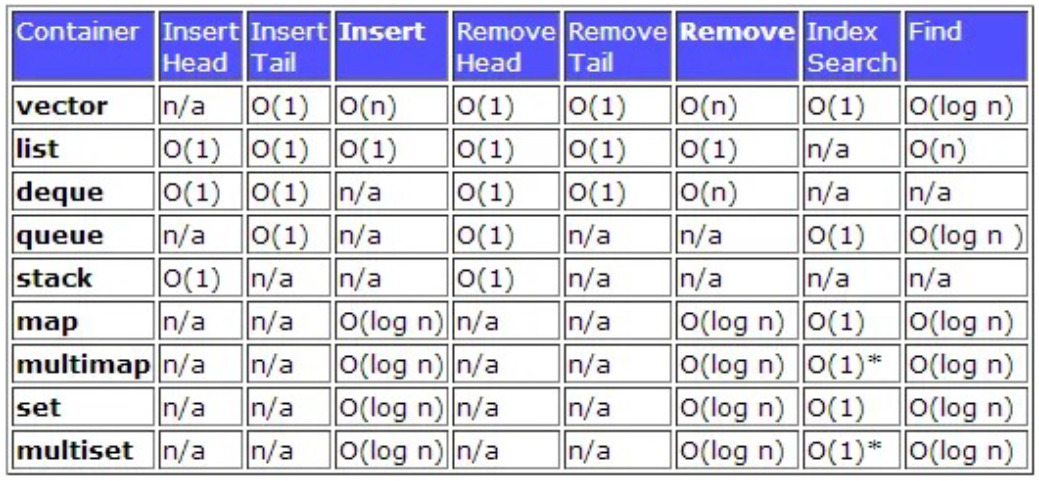
\includegraphics[width=1\textwidth]{Imagen de WhatsApp 2024-11-22 a las 16.47.40_da962cd3.jpg}
\caption{Complejidades Heinz}
\label{fig:mi_imagen} % Puedes referenciar esta imagen más adelante en el documento
\end{figure}


\begin{figure}[h!]
    \centering
    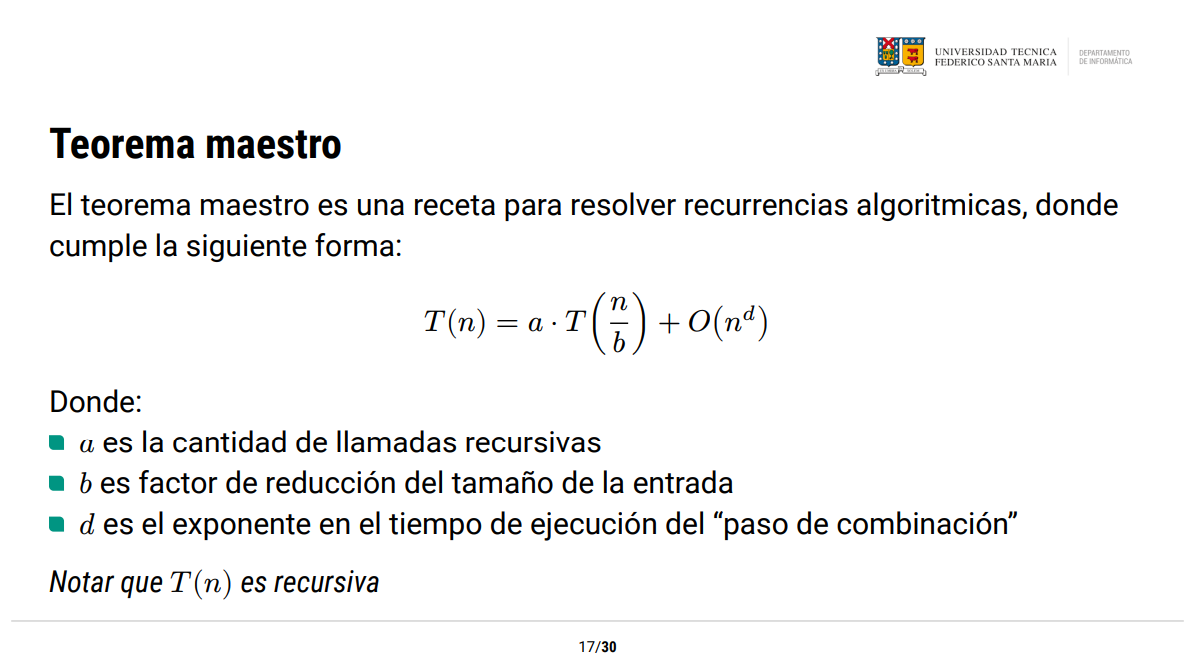
\includegraphics[width=1\linewidth]{imagen_2024-11-22_170622823.png}
    \caption{Teorema Maestro}
    \label{fig:enter-label}
\end{figure}



\begin{figure}[h!]
    \centering
    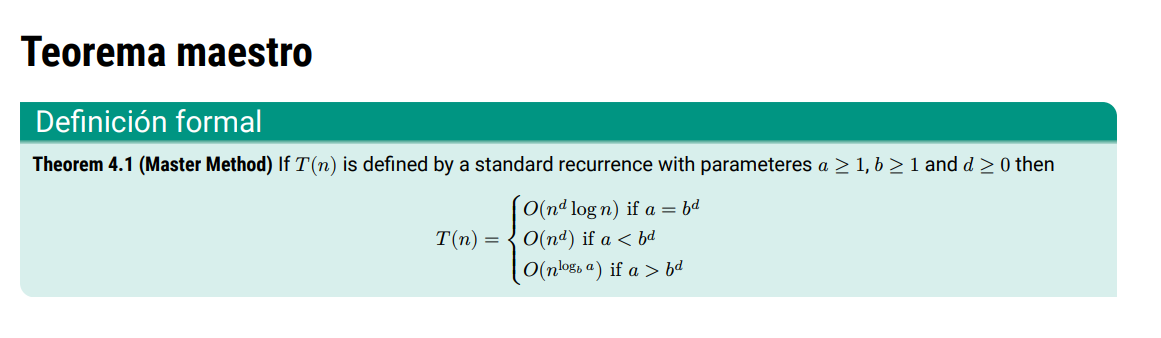
\includegraphics[width=0.7\linewidth]{imagen_2024-11-22_170723408.png}
    \caption{Teorema Maestro Parte 2}
    \label{fig:enter-label}
\end{figure}

\end{document}

